% !TEX program = xelatex
\documentclass[aspectratio=169,10pt]{ctexbeamer}

\usetheme{hkustgzugod}
\usepackage{amssymb}
\usepackage{amsmath}
\usepackage{booktabs}
\usepackage{tabularx}
\usepackage{adjustbox}
\usepackage{listings}
\usepackage{tikz}
\usetikzlibrary{arrows.meta,positioning,shapes.geometric,fit}
\graphicspath{{figures/}}

\title[RoadGen3D]{RoadGen3D：从设计意图到可评价的 3D 街道场景}
\subtitle{Rule/Constraint-Driven, AI-Assisted Street Scene Generation and Evaluation}
\author[王世琦 · GIStudio]{王世琦 \quad GIStudio}
\institute[HKUST(GZ) UGOD]{香港科技大学（广州）社会枢纽\\城市治理与设计学域（UGOD）}
\setsource{GIStudio Internal Project}{2026}
\setdomains{\domaintag{Urban Design}\domaintag{3D Generation}\domaintag{GeoAI}}
\setpresenter{王世琦}
\setvenue{Faculty Project Presentation}
\date{2026-07-10}

\newcommand{\statusdone}{\tikz[baseline=-0.55ex]\node[rounded corners=2pt,fill=hkustblue2,text=white,inner xsep=4pt,inner ysep=1.5pt,font=\tiny\bfseries]{已实现};}
\newcommand{\statuspartial}{\tikz[baseline=-0.55ex]\node[rounded corners=2pt,fill=hkustgold,text=white,inner xsep=4pt,inner ysep=1.5pt,font=\tiny\bfseries]{条件支持};}
\newcommand{\statusnext}{\tikz[baseline=-0.55ex]\node[rounded corners=2pt,fill=hkustgrey,text=white,inner xsep=4pt,inner ysep=1.5pt,font=\tiny\bfseries]{下一步};}
\newcommand{\sourcefoot}[1]{\vfill{\scriptsize\color{hkustgrey}证据来源：\texttt{#1}}}
\newcommand{\artifact}[1]{\texttt{\color{hkustblue2}#1}}
\newcommand{\flowarrow}{\tikz[baseline=-0.4ex]\draw[-{Stealth[length=2mm]},line width=0.8pt,color=hkustgold] (0,0)--(0.5,0);}
\newcommand{\smallclaim}[1]{\par\smallskip{\small\color{hkustblue}\bfseries #1}\par}

\lstset{
  basicstyle=\ttfamily\scriptsize,
  keywordstyle=\color{hkustblue}\bfseries,
  stringstyle=\color{hkustgold},
  commentstyle=\color{hkustgrey},
  showstringspaces=false,
  breaklines=true,
  columns=fullflexible,
  frame=single,
  rulecolor=\color{cardgrey},
  backgroundcolor=\color{bgsoft},
  xleftmargin=2mm,
  xrightmargin=2mm
}

\begin{document}

% -----------------------------------------------------------------------------
\begin{frame}[plain]
  \titlepage
\end{frame}

% -----------------------------------------------------------------------------
\begin{frame}{RoadGen3D 的研究对象是“可审查的生成链路”，不是单纯 3D Viewer}
  \begin{columns}[T,onlytextwidth]
    \column{0.43\textwidth}
      \begin{callout}[一句话定位]
        一个\shl{规则/约束驱动、AI 辅助}的 3D 城市街道场景生成与评价系统。
      \end{callout}
      \tightgap
      \begin{itemize}
        \item 输入如何落到具体道路与设施？
        \item 规则是否满足、失败在哪里？
        \item 不同方案为什么不同、能否复现？
      \end{itemize}
      \smallclaim{核心贡献路径}
      \centering
      \keyword{Design intent} \flowarrow
      \keyword{Explicit IR} \flowarrow
      \keyword{3D artifacts} \flowarrow
      \keyword{Evaluation}
    \column{0.54\textwidth}
      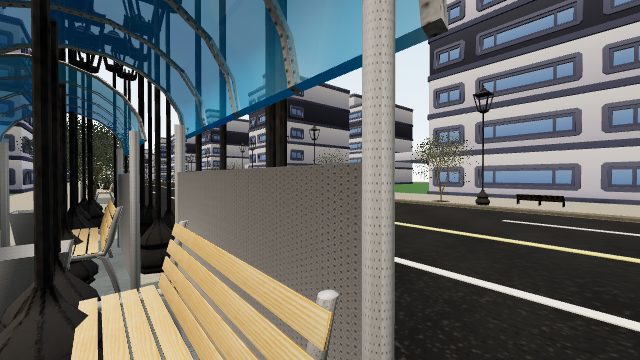
\includegraphics[width=\linewidth,height=0.62\textheight,keepaspectratio]{scene_bus_stop_detail.png}
      \figcap{1}{语义编辑落到公交站棚、座椅、道路与建筑界面；图像只是结果证据之一。}
  \end{columns}
  \sourcefoot{docs/ROADGEN3D\_FRAMEWORK.md; docs/current-progress.md}
  \note{开场不要从“我们做了一个漂亮 Viewer”开始。先把研究对象说成可控、可追踪、可评价的生成链路。}
\end{frame}

% -----------------------------------------------------------------------------
\begin{frame}[plain,c]{系统把设计意图编译成可评价场景，并保留人工审查反馈}
  \centering
  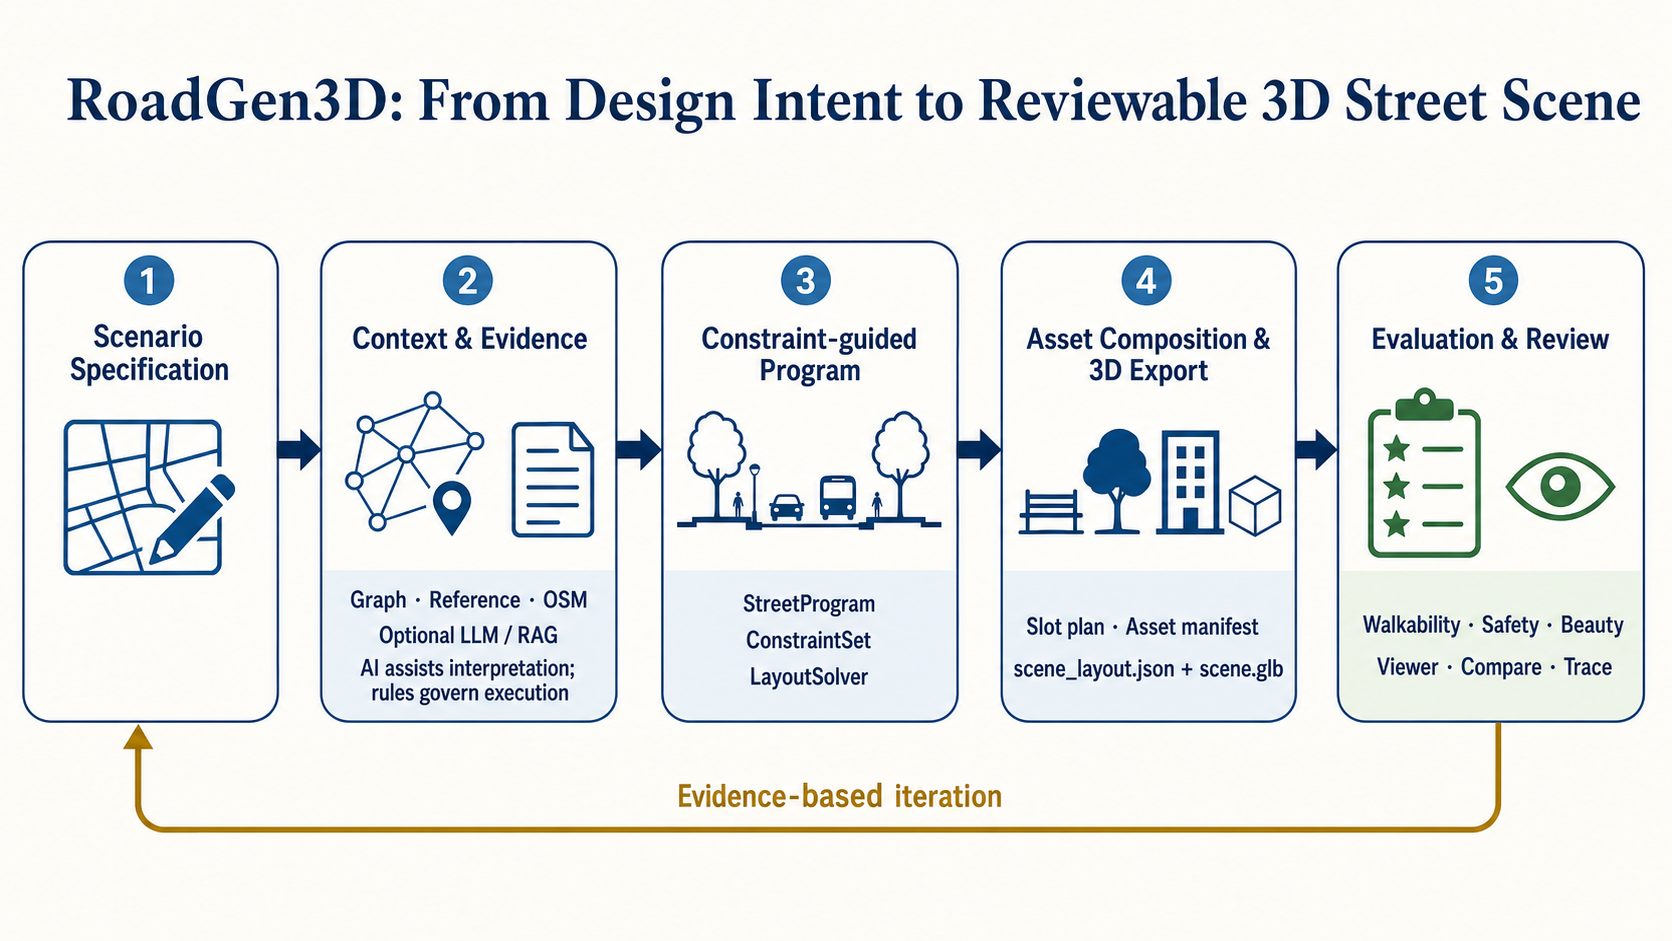
\includegraphics[width=0.97\paperwidth,height=0.78\paperheight,keepaspectratio]{roadgen3d_workflow.png}
  \par\vspace{-1mm}
  {\scriptsize\color{hkustgrey}AI assists interpretation; rules govern execution. 评价反馈回到下一轮场景设定，而不是形成无监督自动决策。}
  \note{用 45 秒讲五阶段：场景设定、上下文与证据、约束程序、资产与导出、评价与审查。}
\end{frame}

% -----------------------------------------------------------------------------
\begin{frame}{显式中间表示把自然语言与 3D 几何隔开}
  \begin{columns}[T,onlytextwidth]
    \column{0.59\textwidth}
      \renewcommand{\arraystretch}{1.12}
      \small
      \begin{tabularx}{\linewidth}{@{}p{0.34\linewidth}X@{}}
        \toprule
        \theadrow \thc{中间表示} & \thc{回答的问题} \\
        \midrule
        \artifact{DesignDraft} & 用户真正要求什么？哪些字段来自显式输入、preset 或证据？ \\
        \altrow \artifact{SceneContext} & 使用 graph template、reference、OSM 还是兼容模板？ \\
        \artifact{StreetProgram} & 道路横断面、功能带、需求与家具目标如何表达？ \\
        \altrow \artifact{ConstraintSet} & 哪些是 hard rule，哪些是 soft objective？ \\
        \artifact{LayoutSolverResult} & band 宽度、slot plan、冲突与 fallback 是什么？ \\
        \altrow \artifact{scene\_layout.json} & 哪些事实可供 Viewer、评价、diff 与复现共同消费？ \\
        \bottomrule
      \end{tabularx}
    \column{0.38\textwidth}
      \begin{callout}[为何不直接 prompt-to-mesh？]
        街道设计需要保留\shl{人行净宽、公交边缘、家具间距、安全岛、碰撞与规则证据}；这些都不能只靠最终网格解释。
      \end{callout}
      \tightgap
      \begin{exampleblock}{两个输出、两种角色}
        \begin{itemize}
          \item \artifact{scene.glb}：渲染与交换载体
          \item \artifact{scene\_layout.json}：事实与评价契约
        \end{itemize}
      \end{exampleblock}
  \end{columns}
  \sourcefoot{docs/DATA\_CONTRACTS.md; src/roadgen3d/services/design\_types.py; src/roadgen3d/types.py}
\end{frame}

% -----------------------------------------------------------------------------
\begin{frame}{AI 负责解释与取证，确定性规则负责落地}
  \begin{columns}[T,onlytextwidth]
    \column{0.31\textwidth}
      \begin{block}{AI / RAG 辅助层}
        \begin{itemize}
          \item 意图解析与检索 query
          \item PDF / GraphRAG / 参数 triples
          \item 参数建议与字段级 citation
          \item 可选视觉评价与改进建议
        \end{itemize}
      \end{block}
    \column{0.31\textwidth}
      \begin{alertblock}{规则与契约层}
        \begin{itemize}
          \item compose patch 白名单
          \item template patch 验证
          \item hard / soft constraints
          \item 几何、碰撞、道路侵入 veto
        \end{itemize}
      \end{alertblock}
    \column{0.31\textwidth}
      \begin{exampleblock}{可追溯输出}
        \begin{itemize}
          \item 最终值与来源优先级
          \item citations / overridden candidates
          \item requested / used backend
          \item fallback reason 与 warnings
        \end{itemize}
      \end{exampleblock}
  \end{columns}
  \deckgap
  \begin{callout}[关键不变量]
    \shl{Manual / explicit input} 的优先级高于 LLM 建议；learned 或 RAG 不可用时必须记录 fallback，不能静默替换。
  \end{callout}
  \sourcefoot{src/roadgen3d/llm/design\_workflow.py; src/roadgen3d/services/design\_runtime.py; generation\_trace.json}
\end{frame}

% -----------------------------------------------------------------------------
\begin{frame}{道路骨架先限定空间，solver 再把需求编译成槽位计划}
  \begin{columns}[T,onlytextwidth]
    \column{0.48\textwidth}
      \begin{block}{1. Graph / Reference Bridge}
        base annotation + \artifact{template\_patch}
        \flowarrow RoadSegmentGraph + PlacementContext
      \end{block}
      \tightgap
      \begin{block}{2. Program + Constraints}
        \artifact{StreetProgram} 描述 bands、需求和目标；\artifact{ConstraintSet} 编译设计规则。
      \end{block}
      \tightgap
      \begin{block}{3. Layout Solver}
        输出 band widths、slot plans、rule evaluations、conflicts 与 fallback provenance。
      \end{block}
    \column{0.49\textwidth}
      \begin{tikzpicture}[x=0.68cm,y=0.68cm]
        \fill[bgsoft] (0,0) rectangle (8,5.2);
        \fill[hkustgoldbg] (0.3,0.4) rectangle (1.5,4.8);
        \fill[cardgrey] (1.5,0.4) rectangle (2.5,4.8);
        \fill[hkustblue2!80] (2.5,0.4) rectangle (5.5,4.8);
        \fill[cardgrey] (5.5,0.4) rectangle (6.5,4.8);
        \fill[hkustgoldbg] (6.5,0.4) rectangle (7.7,4.8);
        \draw[white,dashed,line width=1pt] (4,0.5)--(4,4.7);
        \draw[hkustblue,line width=0.8pt] (0.3,0.4) rectangle (7.7,4.8);
        \node[rotate=90,font=\scriptsize\bfseries] at (0.9,2.6) {Frontage};
        \node[rotate=90,font=\scriptsize\bfseries] at (2.0,2.6) {Sidewalk};
        \node[rotate=90,text=white,font=\scriptsize\bfseries] at (3.3,2.6) {Lane};
        \node[rotate=90,text=white,font=\scriptsize\bfseries] at (4.7,2.6) {Lane};
        \node[rotate=90,font=\scriptsize\bfseries] at (6.0,2.6) {Sidewalk};
        \node[rotate=90,font=\scriptsize\bfseries] at (7.1,2.6) {Furniture};
        \foreach \x in {6.8,7.15,7.5}{\fill[hkustteal] (\x,1.0) circle (0.11);}
        \node[anchor=west,font=\tiny,text=hkustgrey] at (0.3,5.05) {Cross-section bands + allowed placement zones};
      \end{tikzpicture}
      \begin{callout}[规则示例]
        最低人行净宽、公交站只允许进入 transit edge、座椅避开停靠包络、资产不得侵入 carriageway。
      \end{callout}
  \end{columns}
  \sourcefoot{src/roadgen3d/template\_patch.py; graph\_template\_scene\_bridge.py; design\_rules.py; layout\_solver.py}
\end{frame}

% -----------------------------------------------------------------------------
\begin{frame}{资产不是随机散落：需求、检索、过滤与放置共同决定结果}
  \begin{columns}[T,onlytextwidth]
    \column{0.32\textwidth}
      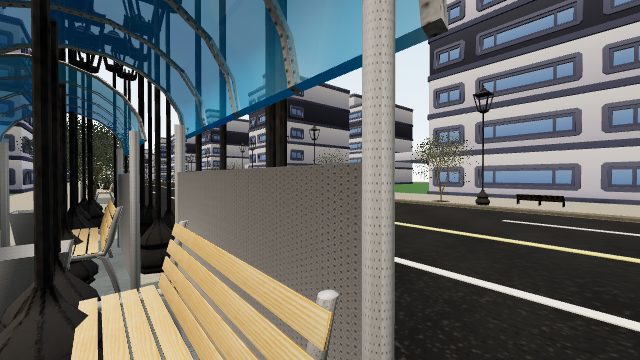
\includegraphics[width=\linewidth]{scene_bus_stop_detail.png}
      \figcap{2}{人尺度：公交站棚与座椅}
    \column{0.32\textwidth}
      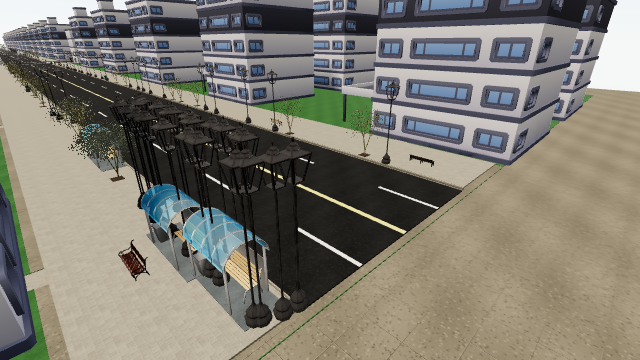
\includegraphics[width=\linewidth]{scene_junction.png}
      \figcap{3}{整体构成：站点、路灯、建筑}
    \column{0.32\textwidth}
      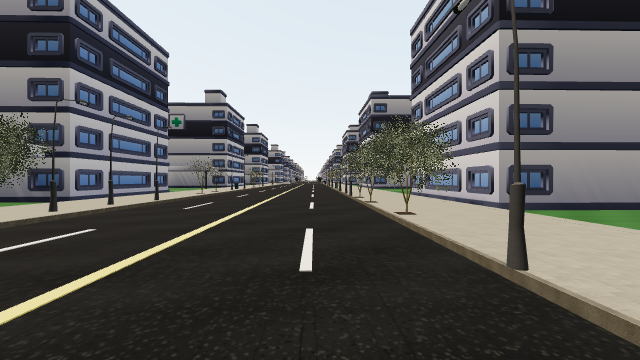
\includegraphics[width=\linewidth]{scene_street.png}
      \figcap{4}{道路连续界面}
  \end{columns}
  \deckgap
  \centering
  \keyword{Furniture requirements}
  \flowarrow \keyword{Slot plan}
  \flowarrow \keyword{Manifest retrieval}
  \flowarrow \keyword{Geometry / rule filters}
  \flowarrow \keyword{Placement + mesh export}
  \deckgap
  \begin{callout}[失败同样是数据]
    未放置资产、碰撞、道路侵入、side mismatch 与 constraint veto 被保留为 diagnostics，而不是强行塞入场景。
  \end{callout}
  \sourcefoot{src/roadgen3d/street\_layout.py; placement\_decisions.jsonl; capture\_manifest.json}
\end{frame}

% -----------------------------------------------------------------------------
\begin{frame}{Plan、GLB 与 trace 共同构成可复现的场景证据}
  \begin{columns}[T,onlytextwidth]
    \column{0.60\textwidth}
      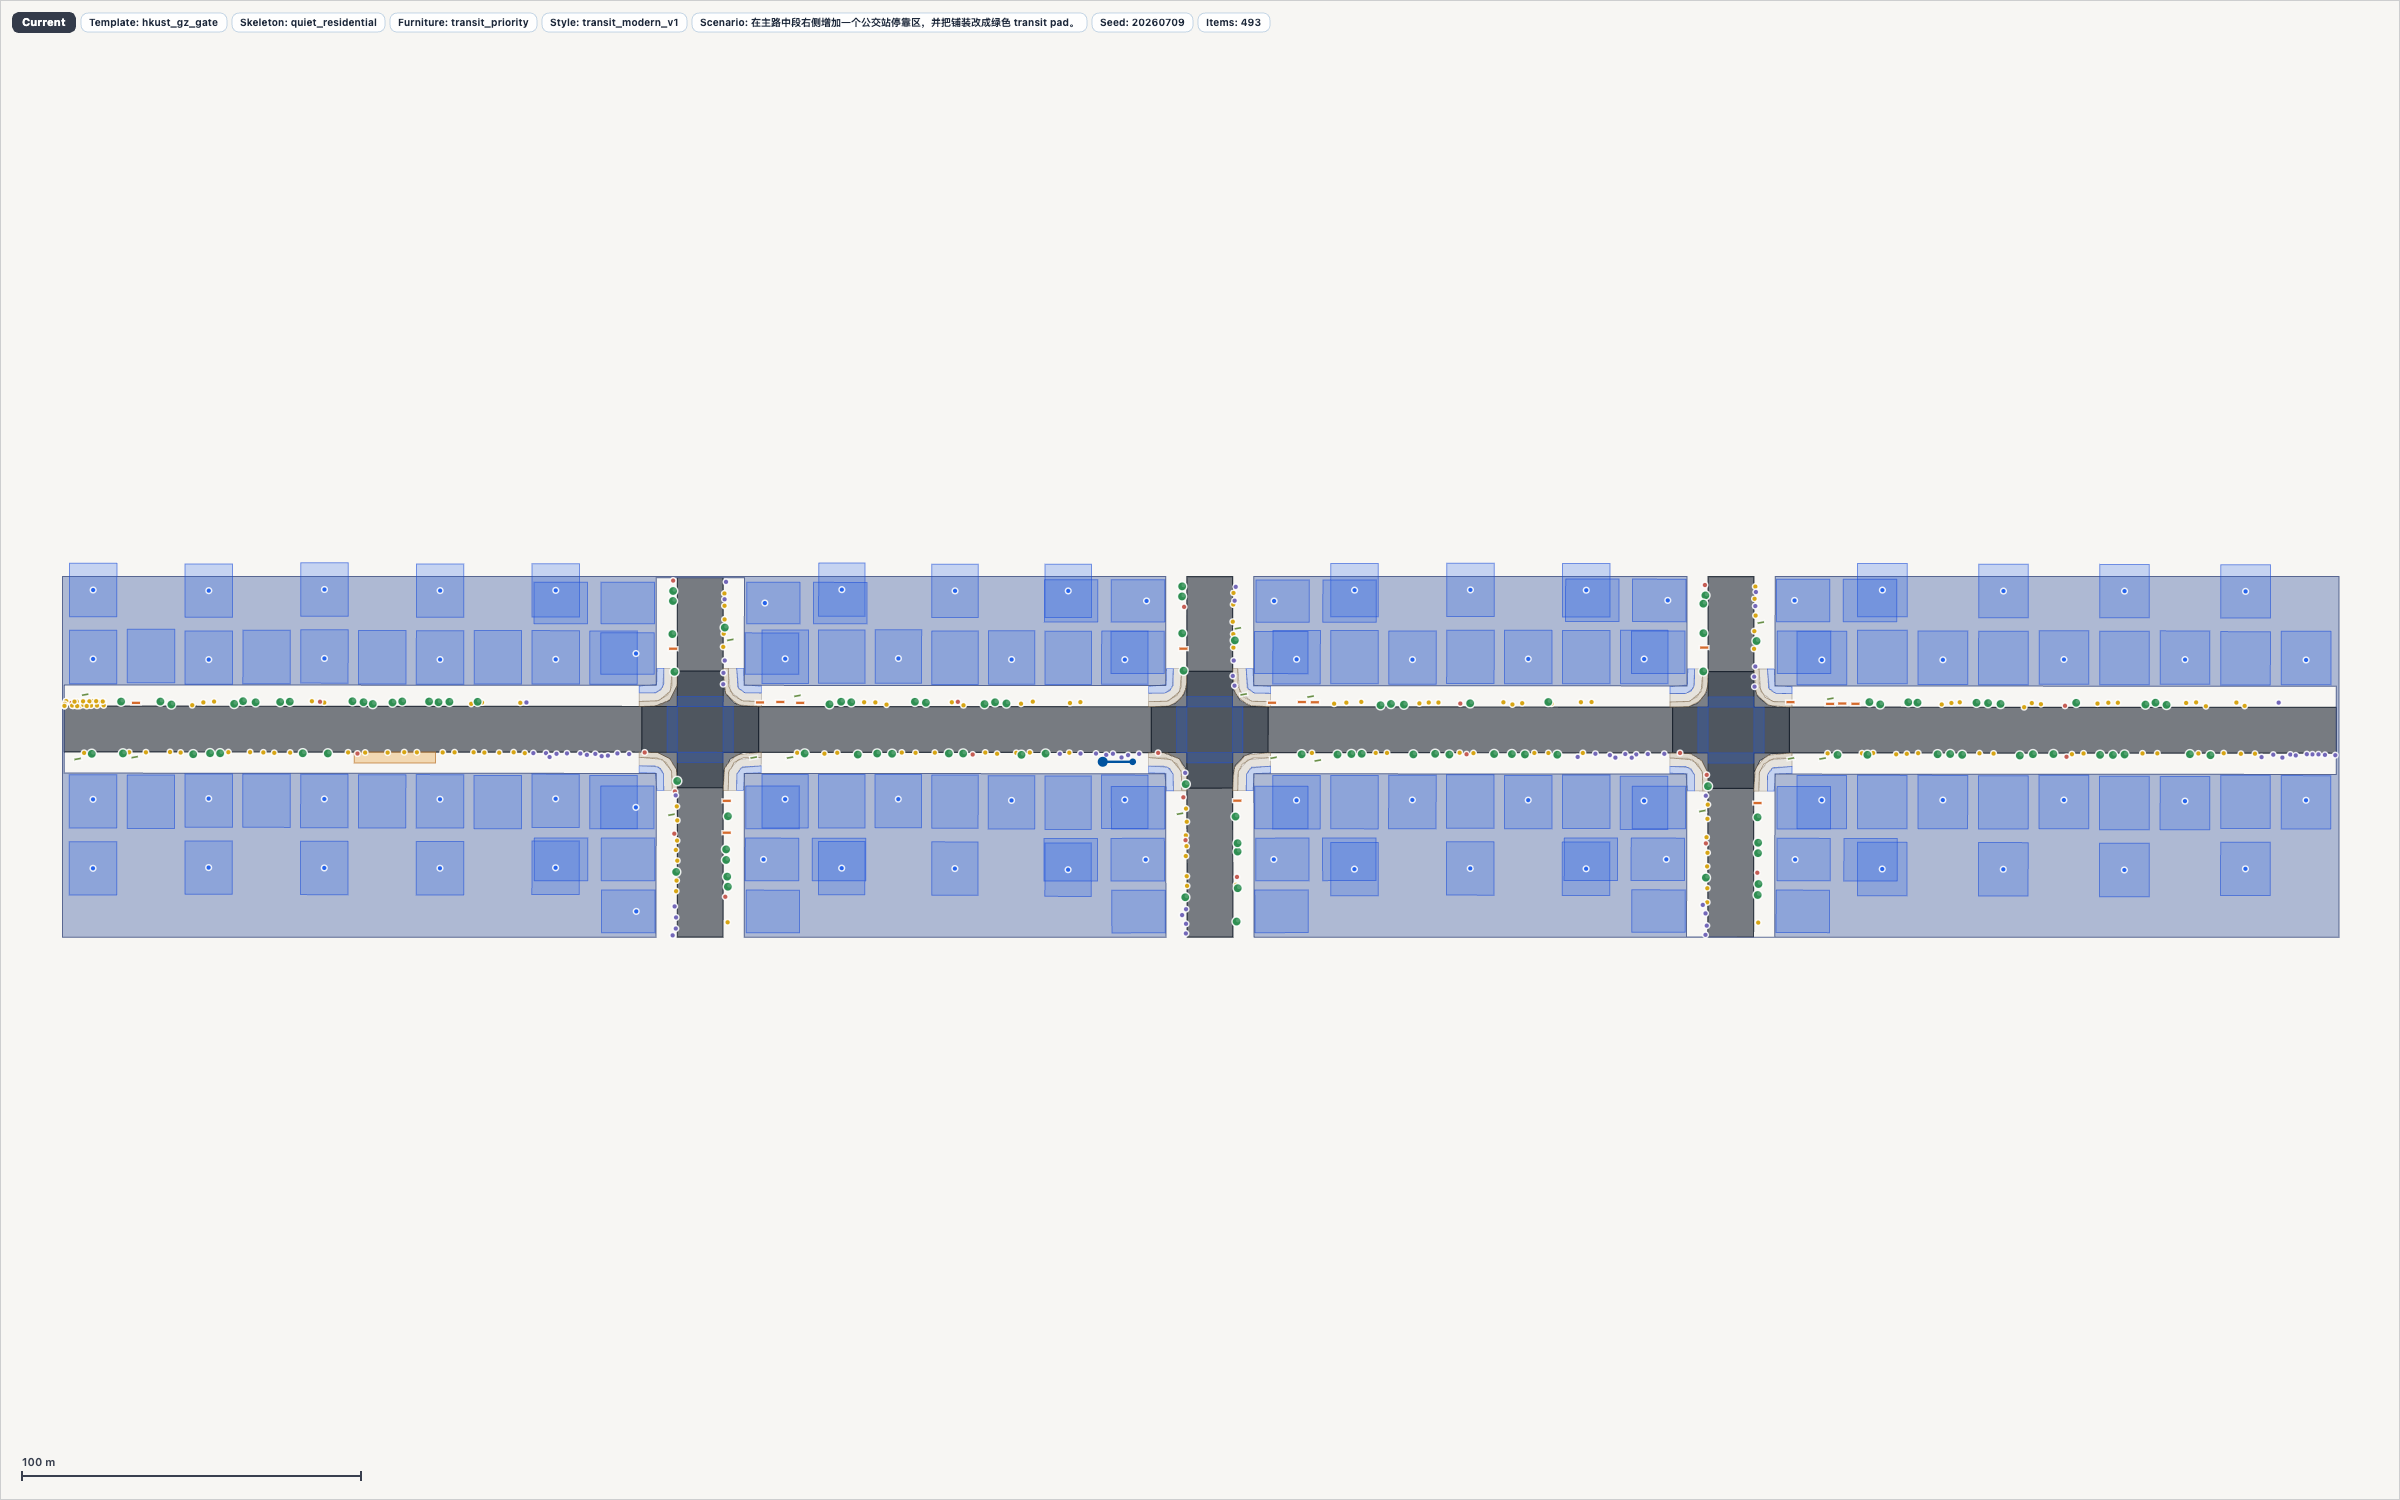
\includegraphics[width=\linewidth,trim=0 450 0 250,clip]{scene_plan_map.png}
      \figcap{5}{Scene Map Plan：道路、surface、建筑与家具由同一 manifest 驱动。}
    \column{0.37\textwidth}
      \begin{exampleblock}{建议交付的 run 目录}
        \begin{itemize}
          \item \artifact{scene\_layout.json}
          \item \artifact{scene.glb}
          \item \artifact{generation\_trace.json}
          \item \artifact{production\_steps/}
          \item \artifact{placement\_decisions.jsonl}
          \item \artifact{view\_captures/}
        \end{itemize}
      \end{exampleblock}
      \tightgap
      \begin{callout}[主数据原则]
        GLB 可以重建或替换；\shl{layout + provenance} 才能解释场景从哪里来。
      \end{callout}
  \end{columns}
  \sourcefoot{artifacts/full\_flow\_smoke/.../20260709T153713Z; web/viewer/src/viewer-api.ts}
\end{frame}

% -----------------------------------------------------------------------------
\begin{frame}{评价把结构化证据与视觉证据分开，并对缺失输入诚实降级}
  \begin{columns}[T,onlytextwidth]
    \column{0.47\textwidth}
      \begin{block}{结构化证据}
        \artifact{scene\_layout.json}
        \begin{itemize}
          \item 横断面与净宽
          \item slot / placement / overlap
          \item 规则满足、冲突与可行性
          \item Walkability 与 generation quality
        \end{itemize}
      \end{block}
    \column{0.47\textwidth}
      \begin{exampleblock}{视觉证据（可选）}
        Rendered views / capture manifest
        \begin{itemize}
          \item Safety / Beauty 视觉判断
          \item 多视角、儿童视角、overview
          \item LLM status 与 visual input 状态
          \item 场景特定 rubric / semantic gates
        \end{itemize}
      \end{exampleblock}
  \end{columns}
  \deckgap
  \begin{callout}[评价诚信规则]
    没有有效 rendered views 或 evaluator 时，Safety / Beauty / Overall 显示为 \shl{N/A}，而不是把缺失证据伪装成 0 分或完整总分。
  \end{callout}
  \sourcefoot{docs/EVALUATION.md; viewer-evaluation-runner.ts; eval\_engine\_ext/road\_metrics}
\end{frame}

% -----------------------------------------------------------------------------
\begin{frame}{面向老师的现场展示应在 4 分钟内完成“意图—机制—结果—评价”}
  \begin{columns}[T,onlytextwidth]
    \column{0.60\textwidth}
      \begin{enumerate}
        \item[\textbf{0:00}] \shl{定性}：Viewer 只是审查载体，先展示最终场景与 production steps。
        \item[\textbf{0:35}] \shl{编辑}：输入“主路中段右侧增加 24 m 绿色公交站台”。
        \item[\textbf{1:15}] \shl{编译}：展示 semantic edit、resolved defaults 与 validated template patch。
        \item[\textbf{1:55}] \shl{作业}：提交 job，展示单调进度、stage tree 与 parameter decisions。
        \item[\textbf{2:40}] \shl{审查}：加载预生成 layout，切换 Plan / 3D / production steps。
        \item[\textbf{3:25}] \shl{评价}：展示指标、N/A 降级、compare 与 trace。
      \end{enumerate}
    \column{0.37\textwidth}
      \begin{callout}[现场预热]
        \texttt{make api}\\
        \texttt{make viewer-web}\\
        \texttt{GET /api/health}
      \end{callout}
      \tightgap
      \begin{exampleblock}{失败预案}
        \begin{itemize}
          \item LLM 不可用：\texttt{use\_llm:false}
          \item 生成较慢：切预生成 artifact
          \item visual score 缺失：只讲 structural evidence
          \item job 重启丢失：直接加载磁盘 layout
        \end{itemize}
      \end{exampleblock}
  \end{columns}
  \sourcefoot{Makefile; docs/DEPLOYMENT\_AND\_JOBS.md; semantic\_scenario\_edits.py}
\end{frame}

% -----------------------------------------------------------------------------
\begin{frame}{协作者通过明确契约接入，而不是绕过中间表示直接改 mesh}
  \renewcommand{\arraystretch}{1.18}
  \begin{adjustbox}{max totalsize={\textwidth}{0.68\textheight},center}
  \begin{tabularx}{\textwidth}{@{}p{0.19\textwidth}p{0.26\textwidth}X p{0.21\textwidth}@{}}
    \toprule
    \theadrow \thc{协作角色} & \thc{推荐入口} & \thc{主要输入 / 输出} & \thc{必须保留的边界} \\
    \midrule
    规划 / 设计 & Scenario catalog、semantic edit、template patch & scenario intent、functional zones、surface annotations & 不直接写 mesh；patch 必须验证 \\
    \altrow API / 应用 & \texttt{/api/design/draft}、\texttt{/api/scene/jobs} & JSON request、job polling、result / trace & Draft 与 SceneContext 分离 \\
    生成算法 & Program、Constraint、Solver、asset backend & IR、slot plan、candidate / placement logs & requested / used backend 与 fallback \\
    \altrow 评价 / 分析 & \texttt{scene\_layout.json}、rendered views & metrics、rubric、compare、improvement patch & 缺视觉证据时不得伪造分数 \\
    前端 / 外部工具 & Viewer \texttt{?layout=}、RoadPen bridge & ViewerManifest、GLB、bridge summary / losses & Vite file API 仅本地；bridge 降级可审计 \\
    \bottomrule
  \end{tabularx}
  \end{adjustbox}
  \sourcefoot{docs/ACTIVE\_ENTRYPOINTS.md; tools/bridge/README.md; web/api/schemas.py}
\end{frame}

% -----------------------------------------------------------------------------
\begin{frame}[fragile]{最小 API 合同：提交结构化作业，轮询状态，读取 artifacts}
  \begin{columns}[T,onlytextwidth]
    \column{0.56\textwidth}
\begin{lstlisting}[language=bash]
# 1. create
curl -X POST http://127.0.0.1:8010/api/scene/jobs \
  -H 'Content-Type: application/json' \
  --data-binary @scene_job.json
# -> {"job_id":"...", "status":"queued"}

# 2. poll
curl http://127.0.0.1:8010/api/scene/jobs/$JOB_ID
# -> status, stage, progress, operations,
#    result, evaluation, trace
\end{lstlisting}
    \column{0.40\textwidth}
      \begin{block}{Create request}
        \begin{itemize}
          \item \artifact{draft}
          \item \artifact{scene\_context}
          \item \artifact{patch\_overrides}
          \item \artifact{generation\_options}
        \end{itemize}
      \end{block}
      \tightgap
      \begin{exampleblock}{Success result}
        \begin{itemize}
          \item layout / GLB / PLY paths
          \item summary + compose config
          \item viewer URL
          \item generation trace + evaluation
        \end{itemize}
      \end{exampleblock}
  \end{columns}
  \sourcefoot{POST /api/scene/jobs; GET /api/scene/jobs/\{job\_id\}; src/roadgen3d/services/scene\_jobs.py}
\end{frame}

% -----------------------------------------------------------------------------
\begin{frame}{当前系统已经证明“可控生成链路”，但还没有证明完整道路工程能力}
  \begin{columns}[T,onlytextwidth]
    \column{0.47\textwidth}
      \begin{block}{\statusdone\ 当前可演示}
        \begin{itemize}
          \item Scenario catalog / semantic edit / graph template
          \item 显式 IR、hard/soft rules、slot solver
          \item 资产检索、碰撞过滤、GLB + layout
          \item Viewer Plan / 3D / compare / history
          \item 结构化评价、可选视觉评价、trace
        \end{itemize}
      \end{block}
    \column{0.47\textwidth}
      \begin{exampleblock}{\statuspartial\ 条件或实验能力}
        \begin{itemize}
          \item LLM / PDF RAG / GraphRAG 依赖配置与 artifacts
          \item learned program / placement 依赖 checkpoint 与 runtime
          \item Safety / Beauty 依赖有效视觉输入
          \item OSM / MetaUrban / reference 路径尚需契约收敛
        \end{itemize}
      \end{exampleblock}
  \end{columns}
  \deckgap
  \begin{callout}[\statusnext\ 当前不能过度宣称]
    尚未覆盖完整 lane movement、signal/control、交通仿真、生产级多用户任务系统，也不能把显式结构直接等同于已验证的“神经符号模型”。
  \end{callout}
  \sourcefoot{docs/current-progress.md; docs/DEPLOYMENT\_AND\_JOBS.md; docs/ROADGEN3D\_FRAMEWORK.md}
\end{frame}

% -----------------------------------------------------------------------------
\begin{frame}{下一阶段应先证明有效性，再扩大模型与道路工程复杂度}
  \begin{enumerate}
    \item \shl{固定 benchmark 与 golden artifacts}\par
      场景、seed、asset manifest、rendered views、评价 profile 与预期结果全部可复现。
    \item \shl{增强道路工程评价}\par
      lane connectivity、turn movements、crossing exposure、reachability、delay 与 simulation-based safety。
    \item \shl{再评估学习能力的必要性}\par
      只有补齐训练数据、checkpoint、baseline、消融与 Viewer 主线闭环后，才提升 learned / neuro-symbolic claim。
  \end{enumerate}
  \deckgap
  \begin{callout}[希望老师重点反馈]
    \begin{itemize}
      \item 首个 benchmark 应优先证明：\keyword{规则满足}、\keyword{设计差异}，还是\keyword{评价稳定性}？
      \item 当前最有研究价值的接口是 scenario specification、constraint solver，还是 evaluation protocol？
    \end{itemize}
  \end{callout}
  \sourcefoot{README.md Roadmap; docs/EVALUATION.md; docs/current-progress.md}
\end{frame}

% -----------------------------------------------------------------------------
\begin{frame}[plain,c]
  \centering
  {\fontsize{38}{42}\selectfont\bfseries\color{hkustblue} RoadGen3D}
  \deckgap
  {\Large 从设计意图到\shl{可控、可追溯、可评价}的 3D 街道场景}
  \deckgap
  {\large\color{hkustgrey}Q\,\&\,A}
\end{frame}

% ============================= Appendix =======================================
\appendix

\begin{frame}{附录 A：关键数据契约与事实输出}
  \renewcommand{\arraystretch}{1.14}
  \begin{tabularx}{\textwidth}{@{}p{0.25\textwidth}X p{0.22\textwidth}@{}}
    \toprule
    \theadrow \thc{契约} & \thc{核心内容} & \thc{主要消费者} \\
    \midrule
    \artifact{DesignDraft} & normalized query、config patch、citations、risk、parameter sources & design runtime \\
    \altrow \artifact{SceneContext} & layout mode、graph/reference/OSM、scenario、template patch & context bridge \\
    \artifact{StreetProgram} & cross-section、demands、furniture requirements、objectives & constraint compiler \\
    \altrow \artifact{ConstraintSet} & declarative hard/soft rules、profile、weights & layout solver \\
    \artifact{LayoutSolverResult} & band solution、slot plans、conflicts、fallback provenance & placement / trace \\
    \altrow \artifact{scene\_layout.json} & config、IR、placements、semantic layers、outputs、summary、scene graph & Viewer / evaluation / diff \\
    \bottomrule
  \end{tabularx}
\end{frame}

\begin{frame}{附录 B：当前最重要的接口}
  \begin{columns}[T,onlytextwidth]
    \column{0.48\textwidth}
      \begin{block}{Generation}
        \begin{itemize}
          \item \texttt{POST /api/design/draft}
          \item \texttt{POST /api/scene/jobs}
          \item \texttt{GET /api/scene/jobs/\{id\}}
          \item \texttt{POST /api/scenario-designs/runs}
          \item \texttt{POST /api/scenario-designs/draft-variant}
        \end{itemize}
      \end{block}
    \column{0.48\textwidth}
      \begin{exampleblock}{Review / Integration}
        \begin{itemize}
          \item \texttt{POST /api/design/evaluate/unified}
          \item \texttt{POST /api/design/evaluate/compare}
          \item \texttt{POST /api/design/capture-views}
          \item Viewer \texttt{?layout=<scene\_layout.json>}
          \item \texttt{tools/bridge/format\_bridge.py}
        \end{itemize}
      \end{exampleblock}
  \end{columns}
  \deckgap
  \begin{callout}[部署边界]
    当前最稳的是同机或共享文件系统下的 HTTP + artifact contract；远程 artifact registry、持久 job table 与 worker pool 尚未生产化。
  \end{callout}
\end{frame}

\begin{frame}{附录 C：最值得老师追问的内部不变量}
  \begin{enumerate}
    \item \shl{Contract separation}：compose patch、SceneContext 与 generation options 不混写。
    \item \shl{Template immutability}：base graph 深拷贝后再 patch，variant 不改源模板。
    \item \shl{IR before geometry}：文本/LLM 不直接摆 mesh。
    \item \shl{Explainable fallback}：requested、used backend 与原因必须同时记录。
    \item \shl{Placement safety}：车行道侵入、碰撞、目标 strip、side 与规则 veto 均需通过。
    \item \shl{Visual-score honesty}：无视觉输入时不返回伪完整分数。
    \item \shl{Artifact duality}：GLB 是视觉载体，layout 是事实契约。
  \end{enumerate}
\end{frame}

\begin{frame}{附录 D：RoadPen 与 RoadGen3D 的桥接边界}
  \begin{columns}[T,onlytextwidth]
    \column{0.46\textwidth}
      \begin{block}{可可靠互通}
        \begin{itemize}
          \item road topology / centerlines
          \item node coordinates / scale
          \item approximate widths / lane counts
          \item geometry-preserving roundtrip checks
        \end{itemize}
      \end{block}
    \column{0.48\textwidth}
      \begin{exampleblock}{可能降级但必须显式记录}
        \begin{itemize}
          \item regions / building regions
          \item surface annotations
          \item station strips / junction composition
          \item furniture relationships
          \item warnings、losses、repaired、\texttt{\_\_bridge\_meta}
        \end{itemize}
      \end{exampleblock}
  \end{columns}
  \deckgap
  \begin{callout}[原则]
    桥接目标是\shl{几何优先、语义降级可审计}，不是声称全语义无损转换。
  \end{callout}
\end{frame}

\end{document}
